%%%%%%%%%%%%%%%%%%%%%%%%%%%%%%%%%%%%%%%%%
% Simple Sectioned Essay Template
% LaTeX Template
%
% This template has been downloaded from:
% http://www.latextemplates.com
%
% Note:
% The \lipsum[#] commands throughout this template generate dummy text
% to fill the template out. These commands should all be removed when 
% writing essay content.
%
%%%%%%%%%%%%%%%%%%%%%%%%%%%%%%%%%%%%%%%%%

%----------------------------------------------------------------------------------------
%	PACKAGES AND OTHER DOCUMENT CONFIGURATIONS
%----------------------------------------------------------------------------------------

\documentclass[12pt]{article} % Default font size is 12pt, it can be changed here


\usepackage{polski}
\usepackage[utf8]{inputenc}

\usepackage{geometry} % Required to change the page size to A4
\geometry{a4paper} % Set the page size to be A4 as opposed to the default US Letter
\newgeometry{tmargin=2cm, bmargin=2cm, lmargin=2cm, rmargin=2cm}

\usepackage{graphicx} % Required for including pictures

\usepackage{float} % Allows putting an [H] in \begin{figure} to specify the exact location of the figure
\usepackage{wrapfig} % Allows in-line images such as the example fish picture

\usepackage{lipsum} % Used for inserting dummy 'Lorem ipsum' text into the template

\linespread{1.2} % Line spacing

%\setlength\parindent{0pt} % Uncomment to remove all indentation from paragraphs

\graphicspath{{Pictures/}} % Specifies the directory where pictures are stored
\usepackage{graphicx}

\begin{document}

%----------------------------------------------------------------------------------------
%	TITLE PAGE
%----------------------------------------------------------------------------------------

\begin{titlepage}

\newcommand{\HRule}{\rule{\linewidth}{0.5mm}} % Defines a new command for the horizontal lines, change thickness here

\center % Center everything on the page

\textsc{\LARGE Politechnika Wrocławska}\\[1.5cm] % Name of your university/college
\textsc{\Large Praca dyplomowa}\\[0.5cm] % Major heading such as course name
\textsc{\large Optimizing routes and commuting time of an ambulance to the victim.}\\[0.5cm] % Minor heading such as course title

\HRule \\[0.4cm]
{ \huge \bfseries 
Optymalizacja drogi i czasu dojazdu karetki pogotowia do poszkodowanego. }\\[0.4cm] % Title of your document
\HRule \\[1.5cm]

\begin{minipage}{0.4\textwidth}
\begin{flushleft} \large
\emph{Autor:}\\
Łukasz \textsc{Joksch}(200963) \\

\end{flushleft}
\end{minipage}
~
\begin{minipage}{0.4\textwidth}
\begin{flushright} \large
\emph{Opiekun:} \\
dr Wojciech \textsc{Kmiecik} % Supervisor's Name
\end{flushright}
\end{minipage}\\[4cm]

{\large \today}\\[3cm] % Date, change the \today to a set date if you want to be precise

%\includegraphics{Logo}\\[1cm] % Include a department/university logo - this will require the graphicx package

\vfill % Fill the rest of the page with whitespace

\end{titlepage}

%----------------------------------------------------------------------------------------
%	TABLE OF CONTENTS
%----------------------------------------------------------------------------------------

\tableofcontents % Include a table of contents

\newpage % Begins the essay on a new page instead of on the same page as the table of contents 

%----------------------------------------------------------------------------------------
%	INTRODUCTION
%----------------------------------------------------------------------------------------

\section{Wstęp}
W swojej pracy chciałbym zaproponować nowy, własny model zarządzania zgłoszeniami ratunkowymi. Aktualny model posiada wiele wad, najpoważniejszą jest fakt, uzależnienia wyboru karetki od jej przynależenia do danej jednostki administracyjnej, nie zawsze jest to optymalny wybór. Przez takie podejście czas oczekiwania na pomoc przez pacjenta wydłuża się. Ponadto, wielokrotnie kierowca, sam decyduje o trasie przejazdu, może wspierać się systemem GPS i nawigacją ale nie ma on pewności, ani wpływu na to czy wybór ten jest optymalny. Decyzja o drodze zostaje podjęta często w chwili, gdy kierowca już prowadzi pojazd, a nie jak intuicyjnie mogłoby wydawać się przed wejściem do karetki przez dedykowany system.
Celem mojej pracy byłoby zaproponowanie nowego modelu wyboru karetki wysyłanej do zgłoszenia oraz implementacja aplikacji wspomagającej tą czynność. W celu przeprowadzenia badań zaimplementowane zostaną różne algorytmy wyboru trasy, uzależniając jej wybór od stopnia zakorkowania danej trasy. Uzyskane wyniki zostaną ze sobą porównane, by w rezultacie wyłonić ten optymalny.
\section{Cel pracy}
W swojej pracy magisterskiej skupię się przedstawieniem problemu dotarcia karetki pogotowia do pacjenta wzywającego pomocy.
Na początku pracy zostanie przedstawiona aktualna sytuacja w naszym kraju dotycząca systemu ratownictwa oraz pokazane zostanie obecne podejście zagospodarowania i organizacji zespołów ratowniczych. W celu uwiarygodnienia, ale przede wszystkim unaocznieniu poruszanego problemu przytoczone zostaną raporty ministerstwa zdrowia i Najwyższej Izby Kontroli (NIK). Zawarte w nich dane pokażą skalę problemu oraz zobrazują obecny model. W swojej pracy postaram pokazać się, iż ten model nie jest optymalny, tj. nie
gwarantuje najszybszego dotarcia do pacjenta w możliwie krótkim czasie. Ponadto system w rozumieniu globalnym działa nierównomiernie, tzn. przy aktualnym gospodarowaniu karetkami w obszarze województwa może dojść do sytuacji, w której w przypadku gdy istnieje wzmożone zapotrzebowanie karetek w jednym województwie, karetki z innego województwa muszą być organizowane na drodze próśb o użyczenie, a nie są brane pod uwagę w momencie zaistnienia zgłoszenia. Dodatkowo należy wspomnieć, iż wykorzystywane mierniki skuteczności zespołów ratowniczych (czas dojazdu do poszkodowanego) niosą za sobą mało informacji.
W swojej pracy będę chciał przedstawić nowy model organizacji karetek pogotowia, czyli taki nie wynikający z stricte z podziałów administracyjnych, a optymalny pod względem czasu i drogi dojazdu z punktu startowego do docelowego.
W kolejnej części swojej pracy dyplomowej zawrę informację o algorytmach optymalizujących drogę. Przedstawione zostaną matematyczne modele oraz pseudokod pokazujący ich programistyczne rozwinięcie. Szczególna uwaga zostanie skupiona na czasie działania każdego algorytmu oraz stopniu trudności jego implementacji i złożoności obliczeniowej.

\section{Zakres pracy}
Rezultatem mojej pracy będzie program komputerowy, w którym owe algorytmy zostaną zaimplementowane. W celach badawczych możliwym będzie wybór, z którego algorytmu program ma w danej chwili korzystać, tj. wyznaczać drogę ze Szpitala do pacjenta. Przewiduje się, że program będzie pobierał dane o korkach drogowych z Internetu, co pozwoli uniknąć zatłoczonych dróg. Będzie to nieocenione dla kierowców. Należy zaznaczyć, iż proponowany program nie będzie jedynie kolejną aplikacją typu GPS, bowiem będzie posiadał zaimplementowaną listę punktów startowych (szpitali, miejsc organizacji karetek pogotowia) i w zależności od miejsca wezwania, sam wybierze z której stacji najlepiej wysłać pogotowie.
Oprogramowanie wspierające symulację, obliczenia i prezentujące wyniki badań zostanie zaprogramowane w języku JAVA, przewiduję powstanie wersji graficznej programu w celu przejrzystej prezentacji badań oraz łatwego poruszania się po jego interfejsie.
Zaimplementowane algorytmy będą porównywane przede wszystkim pod względem czasu pracy, przewidywanego czasu dojazdu karetki do pacjenta oraz długości trasy. Wyniki badań zostaną zapisane do plików w postaci danych tabelarycznych i wykresów. W celu łatwego porównania danej trasy wyniki badań dla każdego algorytmu przedstawione zostaną na jednym wykresie.
Po procesie generowania danych i symulacji przeprowadzona zostanie dogłębna analiza mająca na celu wskazanie optymalnego rozwiązania lub wskazania tego rozwiązania, które na tle pozostałych jest wyjątkowo nieefektywne.
\section{Tematyka pracy dyplomowej - ETAP 3.}

\subsection{Podstawowe Pojęcia}
Tak jak zostało to zasygnalizowane we wstępie głównym celem tej pracy dyplomowej jest wypracowanie nowego modelu zarządzania karetkami pogotowia. Chcąc uczynić proponowane rozwiązanie możliwie najbardziej użytecznym, wygodnym i funkcjonalnym należy dokładnie przyjrzeć się aktualnie działającemu systemowi powiadamiania ratunkowego i jego architekturze. Jest to koniecznym ze względu na to, iż tylko w ten sposób można wychwycić jego wady, niedoskonałości, które mogą zostać poprawione.\\
Chcąc dokładnie przedstawić aktualną architekturę, słowem wstępu, poniżej przedstawiono najważniejsze elementy systemu powiadamiania ratunkowego:
\begin{itemize}
\item 
System 112 - 
Poprzez pojęcie system 112 - jednolity krajowy system odbioru zgłoszeń nanumer alarmowy 112. System ten obejmuje sieć Centrów Powiadamiania Ratunkowego (CPR) - opisane poniżej.Z systemem
współpracują: Policja, Państwowa Straż Pożarna oraz Pogotowie Ratunkowe, a także inne jednostki ratownicze, do których przekierowywane są zgłoszenia alarmowe, które potwierdzają podjęcie akcji ratowniczej lub innej interwencji. Dodatkowo z systemem współpracują publiczni operatorzy sieci telefonicznych oraz
dostawcy ogólnodostępnych usług telekomunikacyjnych.
\item 
Centrum powiadamiania ratunkowego (skrót CPR, ang. public-safety answering point, PSAP) – jednolity system obsługujący zgłoszenia alarmowe kierowane do numerów alarmowych 112, 997, 998 i 999,który  umożliwia przekazanie zgłoszenia alarmowego do odpowiednich służb ratowniczych. 

\item 
Operator 112 - osoba pracująca w CPR, której zadaniem jest odbieranie zgłoszeń od dzwoniących na numer 112, a w następstwie przekazująca je do właściwych służb.
\item 
Dyspozytor - osoba, która dysponuje siłami i środkami pozwalającymi nieść pomoc poszkodowanym w strukturach Policji, Państwowej Straży Pożarnej, Pogotowia Ratunkowego.


\end{itemize}
Centrum powiadamiania ratunkowego (skrót CPR, ang. public-safety answering point, PSAP) – jednolity system obsługujący zgłoszenia alarmowe kierowane do numerów alarmowych 112, 997, 998 i 999,który  umożliwia przekazanie zgłoszenia alarmowego do odpowiednich służb ratowniczych. 

\subsection{Obecny model i architektura Centrum Powiadamiania Ratunkowego}
Aktualne podejście architektoniczne systemu jest podejściem scentralizowanym (choć posiada kilkanaście centrali - jednak połączonych między sobą i ściśle współpracujących), związane z podziałem administracyjnym Polski na województwa. Poszczególne Centra  Powiadamiania Ratunkowego są połączone ze sobą w sieć przy użyciu światłowodów, co pozwala na szybkie przesyłanie danych między tymi ośrodkami. Ponadto dysponują one
% [przypis_duzo_info]
% [potwierdzić informacje informatyczne]
wyspecjalizowanymi serwerami, co jest szczególnie istotną informacją w kontekście tej pracy dyplomowej, gdyż pozwoli to na szybsze działanie proponowanej aplikacji. Platforma aplikacyjna wykorzystywana obecnie pozwala na przesyłanie danych między operatorami 112 a dyspozytorami, dzięki czemu rezultaty pracy aplikacji optymalizującej drogę i czas karetki pogotowia, będą mogły być przekazywane między poszczególnymi jednostkami w postaci plików.
W ramach systemu 112 mamy 16 wojewódzkich Centrów Powiadamiania Ratunkowego. System kooperuje z Platformą Lokalizacyjno-Informacyjną, którą zarządza Urząd Komunikacji Elektronicznej. Poniżej pokazano rozmieszczenie oddziałów CPR na terenie Polski.

\begin{figure}[H]
  \centering
  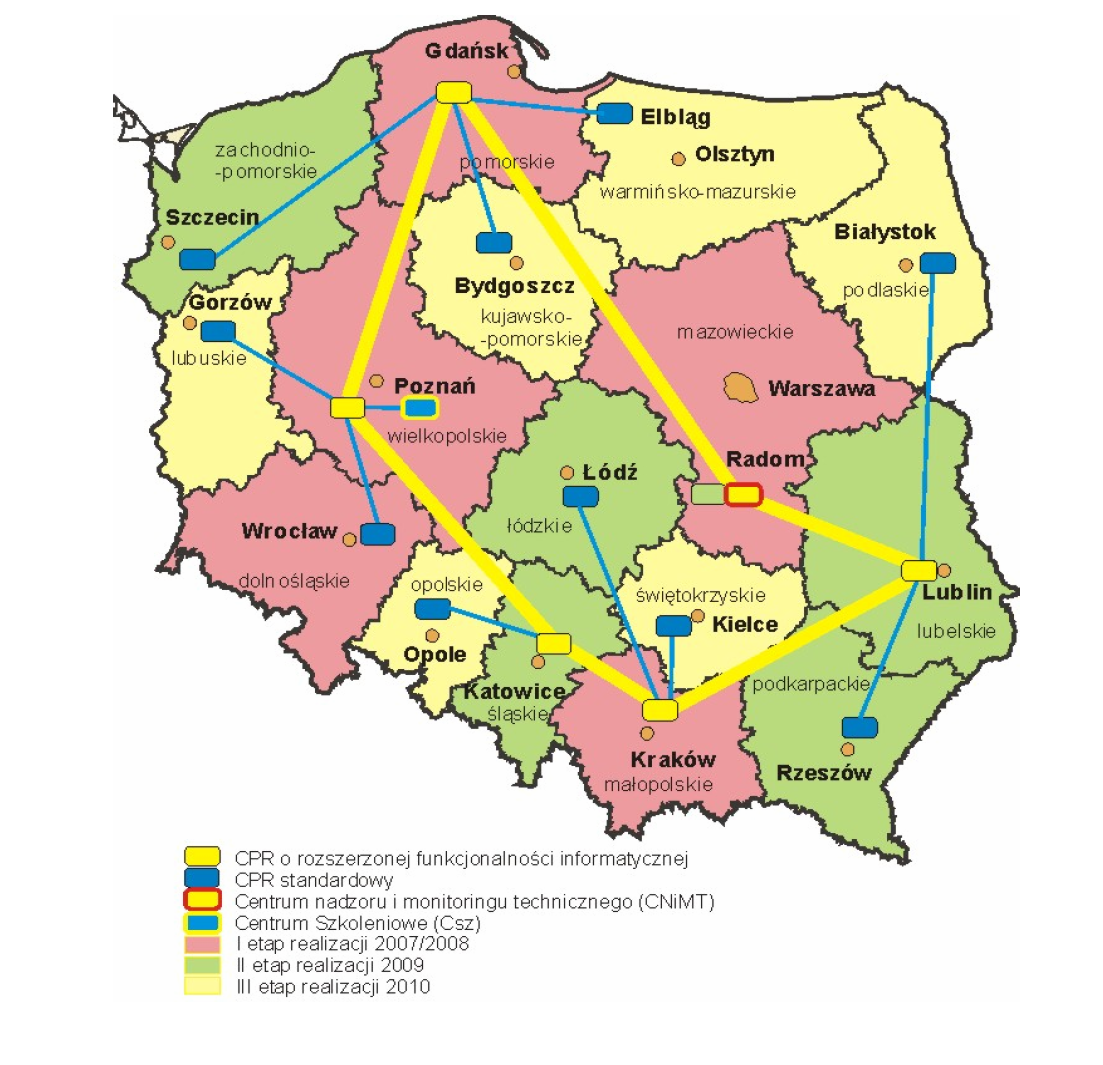
\includegraphics[width=\columnwidth]{images/mapa_cpr.png}
  \caption{Main program view }
\end{figure}






\section{Wstęp}



\newpage
%----------------------------------------------------------------------------------------
%	BIBLIOGRAPHY
%----------------------------------------------------------------------------------------

\begin{thebibliography}{99}
\bibitem{pa} 
Applegate, David L., “The traveling salesman problem : a computational study / David L. Applegate [et al.]”, Princeton ; Oxford : Princeton University Press, cop. 2006.
\bibitem{pa} 
Agnieszka JAKUBOWSKA, Katarzyna PIECHOCKA, „- WYBRANE ALGORYTMY W ZASTOSOWANIU DO PROBLEMU KOMIWOJAŻERA”, JOURNAL OF TRANSLOGISTICS 2015
\bibitem{pa} 
Ivan Brezina Jr., Zuzana Čičková, „Solving the Travelling Salesman Problem Using the Ant Colony Optimization”, Management Information Systems, Vol. 6 (2011), No. 4 pp. 010-014 Received 12 July 2010, Accepted 23 September 2011
\bibitem{pa} 
Neill E. Bowler, Thomas M. A. Fink, Robin C. Ball, “Characterization of the probabilistic traveling salesman problem”, June 13, 2003
\bibitem{pa} 
T.H. Cormen, Ch.E. Leiserson, R.L.Rivest, „Wprowadzenie do algorytmów”, Wyd. Naukowo-Techniczne Warszawa, 2001
\bibitem{pa} 
CHRIS WALSHAW, “A MULTILEVEL APPROACH TO THE TRAVELLING SALESMAN PROBLEM”, London, SE10 9LS, United Kingdom, (Received August 2000; revisions received May 2001, July 2001; accepted August 2001)
\bibitem{pa} 
Christian Blum, “Ant colony optimization: Introduction and recent trends”, ALBCOM, LSI, Universitat Politècnica de Catalunya, Jordi Girona 1-3, Campus Nord, 08034 Barcelona, Spain Accepted 11 October 2005
\bibitem{pa} 
Dweepna Garg and 2Saurabh Shah, „ANT COLONY OPTIMIZATION FOR SOLVING TRAVELING SALESMAN PROBLEM”, International Journal of Computer Science and System Analysis, Vol. 5, No. 1, January-June 2011
\bibitem{pa} 
Koncepcja Systemu 112, MSWiA, Warszawa, wrzesień 2007
\bibitem{pa} 
Encyklopedia Internetowa - Wikipedia, hasło: "Państwowe Ratownictwo Medyczne",
https://pl.wikipedia.org/wiki/Państwowe\_Ratownictwo\_Medyczne
\bibitem{pa} 
Encyklopedia Internetowa - Wikipedia, hasło: "112 (numer alarmowy)",
https://pl.wikipedia.org/wiki/112\_(numer\_alarmowy)




\end{thebibliography}

%----------------------------------------------------------------------------------------

\end{document}